\documentclass{beamer}

\usepackage[pantone312]{wwustyle-moreauthors}

\usepackage[ngerman]{babel}
\usepackage[utf8]{inputenc}
\usepackage[T1]{fontenc}
\usepackage{pgfplotstable}
\usepackage{booktabs}
\usepackage{array}
\usepackage{pgfplots}
\usepackage{lmodern}
\usepackage{media9}
\usepackage{etoolbox}

% Uncomment the following two lines if you want to prepare your document for
% the fast mode.
% \usetikzlibrary{external}
% \tikzexternalize

% If frametitle is empty and subsection is not empty, use subsection as frame title
% If frametitle is empty and subsection is empty, use section as frame title
\makeatletter
  \CheckCommand*\beamer@checkframetitle{%
    \@ifnextchar\bgroup\beamer@inlineframetitle{}}
  \renewcommand*\beamer@checkframetitle{%
    \global\let\beamer@frametitle\relax\@ifnextchar%
    \bgroup\beamer@inlineframetitle{}}
\makeatother

% Reduce TOC margins
\makeatletter
\patchcmd{\beamer@sectionintoc}{\vskip1.5em}{\vskip0.5em}{}{}
\makeatother

\addtobeamertemplate{frametitle}{
  \ifx\insertframetitle\empty
    \ifx\insertframesubtitle\empty
      \ifx\insertsubsection\empty
        \frametitle{\insertsectionhead}
      \else
        \frametitle{\insertsubsectionhead}
      \fi
    \else
    \fi
    \else
    \fi
 }{}

\pgfplotstableset{% global config, for example in the preamble
  every head row/.style={before row=\toprule,after row=\midrule},
  every last row/.style={after row=\bottomrule}
}

% for each new section, show toc with highlighted section name
\AtBeginSection[]
{
  \begin{frame}
    \frametitle{Inhalt}
    \tableofcontents[currentsection,currentsubsection,subsectionstyle=show/show/hide,subsubsectionstyle=hide]
  \end{frame}
}

\author{Robin, Johannes, Alexander}
\title{Emotionserkennung}
% \institutelogo{Logo on title frame}
% \institutelogosmall{Logo on other frames}
\subtitle{Klassifikation von Action Units anhand von Landmarks}
\date{8. September 2016}

\begin{document}

%%%%%%%%%%%%%%% WWUstyle "fast" mode %%%%%%%%%%%%%%%%%%%%%
% Do the following steps in order to speed up the compilation time of your
% presentation:
%
% 1. Include the externalization tikz library in the preamble of your document.
%    This is always recommended if you are using tikz in your document.
% 2. Uncomment the \wwupreparefastmode command below
% 3. Compile your document with command line option '-shell-escape',
%    e.g.: 'pdflatex -shell-escape beamer.tex'
% 4. Comment (or delete) the \wwupreparefastmode
% 5. Add option 'fast' to the 'wwustyle' package declaration line.
% 6. Be happy!

% \wwupreparefastmode


\begin{frame}[plain]
  \maketitle
\end{frame}
\begin{frame}
  \frametitle{Inhalt}
  \tableofcontents[subsectionstyle=hide,subsubsectionstyle=hide]
\end{frame}

\section{Aufgabenstellung}
\subsection{Eingabedaten}
\begin{frame}
  \begin{center}
  \includemedia[
      activate=onclick,
      height=0.8\textheight
  ]{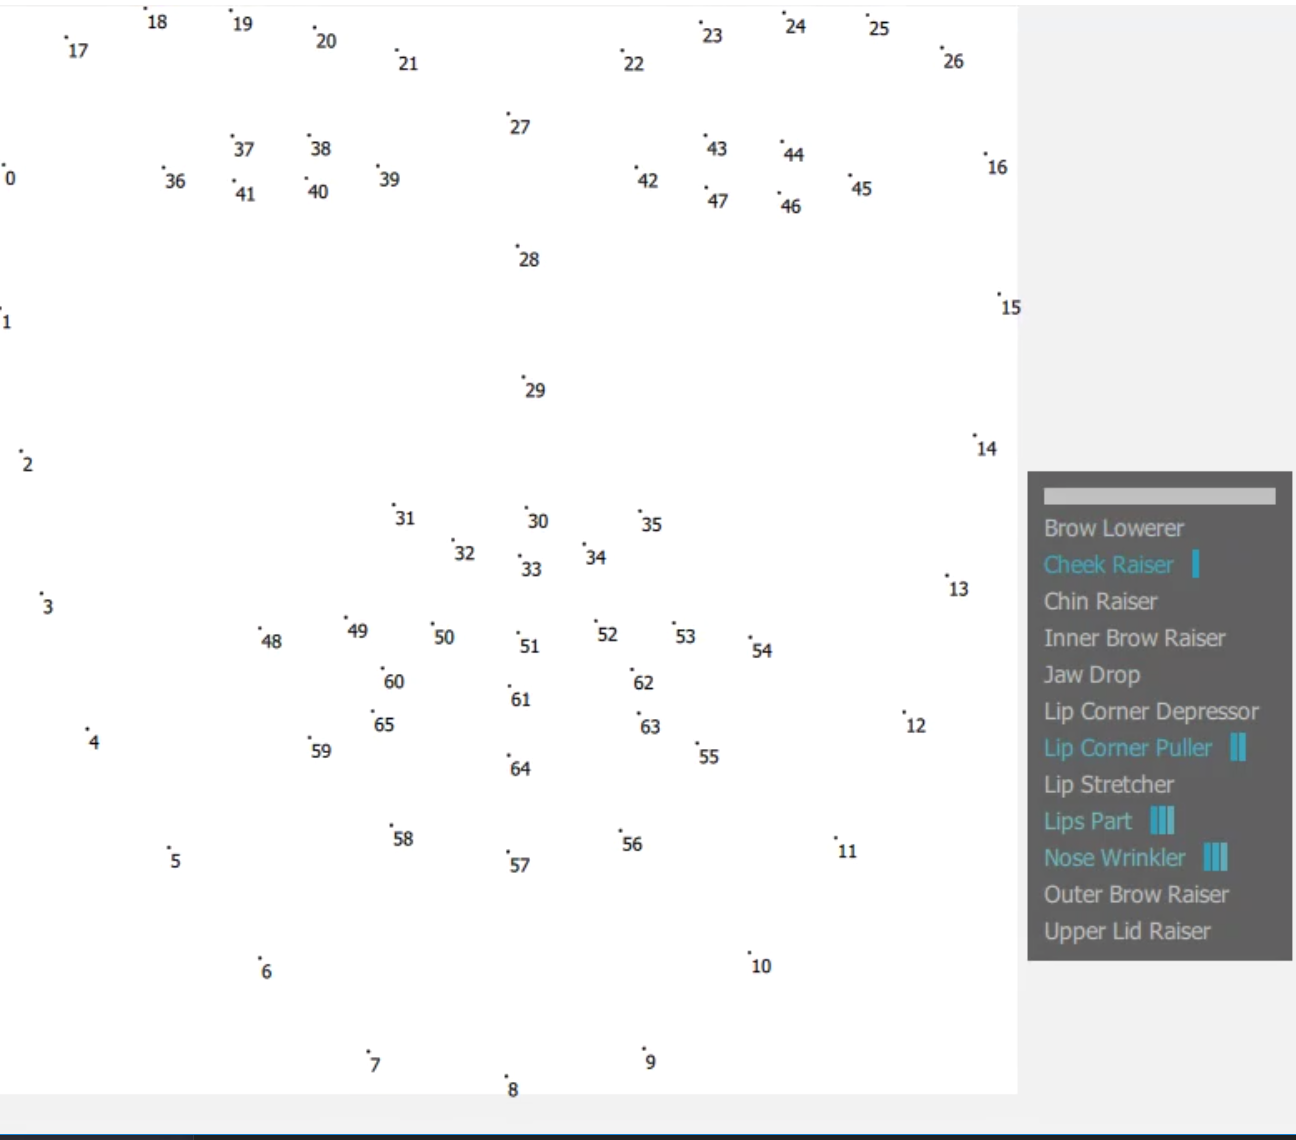
\includegraphics{aufgabenstellung.png}}{aufgabenstellung.swf}
  \end{center}
\end{frame}

\subsection{Ziel}
\begin{frame}
  \begin{block}{Ziel}
    Trainieren eines Klassifikators, der in der Lage ist aus eingehenden Landmarks die aktivierten Action Units zu erkennen.
  \end{block}
\end{frame}

\section{Programmierumgebung}
\begin{frame}
  \begin{itemize}
    \item C++11
    \item OpenCV2
    \item QT5
  \end{itemize}
\end{frame}

\section{Pipeline}
\subsection{Normalisierung}
\begin{frame}
  \begin{itemize}
    \item Problem: Variationen von Position, Skalierung und
      Rotation in den Eingabevideos
    \item Lösung: Normalisierung der Daten
    \begin{itemize}
      \item Zentrieren des Mittelpunktes
      \item Skalierung zwischen 0..1
      \item Rotation mithilfe der Augen
    \end{itemize}
  \end{itemize}
\end{frame}

\subsection{Feature Extraction}
\begin{frame}
  \begin{itemize}
    \item Entwicklung verschiedener Merkmale aus den Landmark-Daten
    \item Beispiel: Relation der Landmarks untereinander
    \item Aufgabe: Extrahierung möglichst aussagekräftiger Merkmale
    \item Schwierigkeit: Aussagekraft der Merkmale vor dem Training unbekannt
  \end{itemize}
\end{frame}

\begin{frame}
\begin{figure}
    \includegraphics[height=0.7\textheight]{feature_extractor.png}
    \caption{FeatureExtractor als Aggregate}
    \end{figure}
\end{frame}

\begin{frame}
\begin{itemize}
  \item Unsere Features:
    \begin{itemize}
      \item X-/Y-Koordinaten
      \item Orientierung
        \begin{itemize}
          \item Paarweise
          \item Zum Mittelpunkt
        \end{itemize}
      \item Euklidische Distanz
        \begin{itemize}
          \item Paarweise
          \item Zum Mittelpunkt
        \end{itemize}
      \item Interpolation
      \item Zeitbasiert
    \end{itemize}
  \end{itemize}
\end{frame}

\subsection{PCA}
\begin{frame}
  \begin{itemize}
    \item $($66 Landmarks$) \times ($\#Features$)$ = teilweise hohe Komplexität\newline
          $\rightarrow$Reduktion der Features auf Hauptkomponenten
    \item Approximation der Daten bei Erhaltung von 97\% der Varianz
    \item Vorsicht: PCA betrachtet die Aussagekraft der Hauptkomponenten bezogen auf die Landmarks, NICHT auf die Erkennung der Action-Units
  \end{itemize}
\end{frame}

\subsection{Feature-Manipulation and -Scaling}
\begin{frame}
  \begin{itemize}
    \item Wenig true-positives in den Eingabedaten\newline
          $\rightarrow$Optional: Generierung zusätzlicher true-positives
    \item Features mit unterschiedlichen Wertebereichen: Rotationsgrad, Distance,...\newline
          $\rightarrow$Normalisierung der Features auf 0..1
  \end{itemize}
\end{frame}

\subsection{Klassifikation}
% \subsubsection{SVM}
\begin{frame}
  \begin{itemize}
    \item Bearbeitete Features werden zum Training an Klassifikatoren übergeben
    \item Klassifikatoren können mit verschiedenen Parametern trainiert werden
    \item Problem erneut: optimale Parameter unbekannt
    \item Unsere Klassifikatoren:
      \begin{itemize}
        \item Support Vector Machine: OpenCV::SVM
        \item Random Forest: OpenCV::CvRTrees
      \end{itemize}
  \end{itemize}
\end{frame}

\subsection{Zusammenfassung}
\begin{frame}[plain]
  \begin{figure}
    \includegraphics[height=\textheight]{pipeline.png}
  \end{figure}
\end{frame}

\section{Evaluation}
\subsection{Methodik}
\begin{frame}
  \begin{itemize}
  \item Erstelle eine Konfigurationsdatei, in der alle zu testenden
    Klassifikatoren und Parameter gespeichert sind (Demo)
  \item Teile ersten Datensatz in $60\%$ Trainings- und $40\%$ Validierungsdaten auf
    \item Trainiere und evaluiere automatisch alle Klassifikatoren auf allen
      Action Units
    \item Wähle pro Action Unit die besten 5 anhand des F1 score aus
    \item Evaluiere Performance auf zweitem Datensatz (bisher unbekannte Testdaten)
  \end{itemize}
\end{frame}
% \begin{frame}
%   % \frametitle{Ein Alerted-Block}
%   \begin{alertblock}{Achtung!}
%     Hier kommt Rot ins Spiel!
%   \end{alertblock}
%   \begin{exampleblock}{Beispiel}
%     Hier kommt Grün ins Spiel!
%   \end{exampleblock}
% \end{frame}

\subsection{Ergebnisse}
\begin{frame}[c]
  % \frametitle{~}
  \begin{center}
    \usebeamerfont*{frametitle}
    \usebeamercolor[fg]{frametitle}
    \Huge Webdemo
  \end{center}
\end{frame}

% \begin{frame}
%   \begin{table}
%   \centering
%   \pgfplotstabletypeset[
%   col sep=comma,
%   columns/Klassifikator/.style={string type}
%   ]{data/tab_prec_recall.csv}
%   \caption{Vergleich der Klassifikatoren}
%   \label{tab:prec-recall}
%   \end{table}
% \end{frame}

% \begin{frame}[plain]
% \begin{figure}
% \begin{tikzpicture}
%   \begin{axis}[
%     width=\textwidth,
%     height=\textheight,
%     xmin=0, xmax=1,
%     ymin=0, ymax=1,
%     xlabel={$1-\text{Precision}$},
%     ylabel={Recall},
%     domain=0:1,
%     % legend entries={Sachen},
%     % legend pos=north west
%   ]
%   \addplot table[only marks, col sep=comma] {data/plt_prec_recall.csv};
%   \end{axis}
% \end{tikzpicture}
% \caption{Precision-Recall-Kurve}
% \label{fig:prec-recall}
% \end{figure}
% \end{frame}
\subsection{Diskussion}
\begin{frame}
  \begin{itemize}
    \item Gute Ergebnisse bei ``Lips Part'', akzeptable bei ``Lip Corner Puller''
      \begin{itemize}
        \item Möglicher Grund: vergleichsweise viele positive Daten (``Lips
          Part'': $8\%$)
        \item Einfache Klassifikation anhand der Abstände der Mund-Landmarks
      \end{itemize}
    \item Schlecht z.B. ``Lip Corner Depressor'': $<0.1\%$ positiv
  \end{itemize}
\end{frame}

\begin{frame}
  \begin{itemize}
    \item Trade-off zwischen Precision und Recall deutlich zu sehen
    \item Klassifikation mit Zeitableitung liefert keine guten Ergebnisse
      \begin{itemize}
        \item Noch weniger positive Daten
      \end{itemize}
    \item Random Forests erfolgreich zusammen mit CenterDistanceExtraction, InterpolationFeatureExtraction
  \end{itemize}
\end{frame}

\subsection{Ausblick}
\begin{frame}
  \begin{itemize}
    \item Verbesserung der Klassifikation durch Kombination von Klassifikatoren
    \item Erkennung von Emotionen, die sich aus mehreren Action Units zusammensetzen
    \item Ausbau der zeitbasierten Features
    \item Weitere Methoden zur Generierung positiver Samples
  \end{itemize}
\end{frame}

\begin{frame}[c]
  \frametitle{~}
  \begin{center}
    \usebeamerfont*{frametitle}
    \usebeamercolor[fg]{frametitle}
    \Huge Ende
  \end{center}
\end{frame}

\end{document}
